\chapter{Resultat}
\paragraph{} Kapittel 4 handler om resultatene fra kapittel-3. Dette kapittelet tar for seg de resultatene som er kommet som følge av gruppens forskning. Her presenteres de ulike resultatene som er funnet samt en arbeidskravs- og en situasjonsanalyse som hjelper prosjektgruppen med å bedre kartlegge det som kreves for å fikse problemet til katoplast.

\section{Arbeidskravsanalyse} 
\paragraph{} Ut i fra informasjonen gruppen hadde tilegnet seg fra Katoplast, utarbeidet prosjektgruppen en arbeidskravsanalyse som skulle ta for seg de viktigste elementene ved en server løsning for å finne den beste løsningen for Katoplast. Gruppen tok for seg en rekke elementer som bedriften satte vekt på, og hvorvidt disse ulike elementene skulle spille inn på hvilke løsninger som skulle analyseres.

\paragraph{}\textbf{Arbeidskravsanalyse som gruppen kom frem til. }
\begin{figure}[H]
\centering
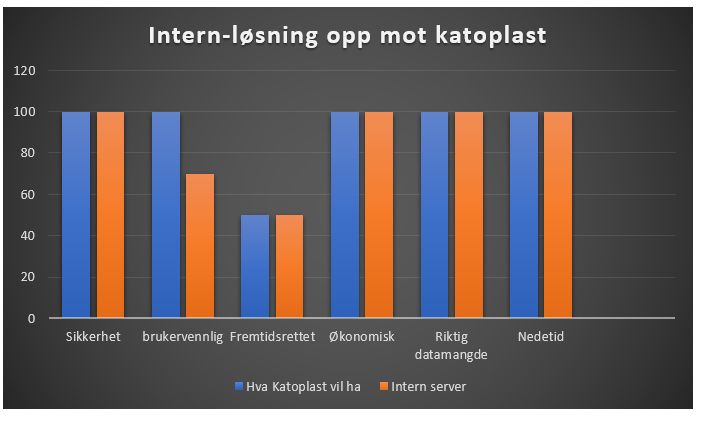
\includegraphics[width=5.5in]{Bilder/abc.PNG}
\caption{Arbeidskravsanalyse}
\end{figure}


\paragraph{Sikkerhet:} \hspace{-0.95em} Sikkerheten til katoplast er det mest fundamentale for bedriften. Bedriften holder på store mengder med sensitiv data som de ønsker å holde hemmelig. Generelt er bedriften avhengig av riktig data for at en normal arbeidsdag skal kunne gå som planlagt. Dersom noe av den sensitive dataen skulle komme på avveie kan bedriften i verste fall gå konkurs. Derfor er sikkerheten på serverløsningene noe av det viktigste og dermed også det gruppen la størst vekt på når de forskjellige løsningene ble analysert. Det er vesentlig at leverandørene tilbyr beskyttelse mot hackere og DDOS-angrep for å unngå nedetid og at sensitiv data ikke skal bli kompromittert. 
\footnote{https://nettvett.no/ddos-angrep/}

\paragraph{}{\bfseries Brukervennlighet:} \hspace{-0.95em}  Det er vesentlig for bedriften å kunne bruke serverne slik de skal brukes. I dag er det dagligleder som står for det meste av drifting og oppdatering av egen server. Dette er oppgaver som daglig leder ønsker å unngå. Det er essensielt at en serverløsning er komfortabel å benytte seg av og tillater enkle metoder for lagring og henting av informasjon og data. Det er også et stort pluss at løsningen tar seg av en rekke administrative oppgaver som ofte krever tid og arbeid når de må gjøres manuelt.  


\paragraph{}{\bfseries Framtidsrettet:} \hspace{-0.95em} Dette kravet tar for seg hvorvidt løsningen er framtidsrettet. Det er nødvendig å tenke om løsningene kan brukes igjennom flere år. Dette kan man tjene på økonomisk. Løsningen til Katoplast i dag er ikke like fremtidsrettet som andre løsninger. Interne servere har blitt brukt i lang tid og vil mest sannsynlig fortsette å brukes i lengre tid fremover, men det er likevel slik at en bør ha et fremtidsrettet syn når det kommer til løsningene. Dette kan lette på det økonomiske trykket og tidspresset som preger katoplast. I midlertid, ønsker ikke bedriften å sette dette kravet for langt oppe på listen og vil nøye seg med en mindre fremtidsrettet løsningen.

\paragraph{}{\bfseries Økonomisk:} \hspace{-0.95em} Økonomisk planlegging og styring er avgjørende i en bedrift. Derfor har gruppen valgt å legge økonomi som et arbeidskrav for løsningen. Det er vesentlig at de ulike serverløsningene som presenteres og analyseres er rimelige når det gjelder pris. Det er vesentlig at kvaliteten på løsningene er høyt, men samtidig hjelper det stort at løsningen ikke er for kostbare. Bedriften er en relativ liten bedrift og har ikke utallige med krav til for avanserte og dyre løsninger.

\paragraph{}{\bfseries Datamengde:} \hspace{-0.95em} Datamengden til bedriften ligger i dag på 500GB. Dette er data de har samlet siden 1972. For at prosjektet skal kunne finne den beste løsningen må man tenke igjennom dataforbruket til bedriften. Ved å finne den riktige datamengden kan dette lette på det økonomiske trykket for bedriften, og samtidig gjøre arbeidet for å finne en løsning lettere for gruppen. 

\paragraph{}{\bfseries Nedetid:} \hspace{-0.95em} For Katoplast var det viktig at deres servere er oppe og kjører hele tiden. De ønsker en løsning hvor serverne har overbevisende sikkerhet til å motstå feil eller andre problemer som kan eventuelt føre til nedetid. Dersom serverne skulle gå ned i lengre tid kan følgene bli katastrofale for katoplast. Bedriften har veldig sjeldent nedetid, derfor er det avgjørende at løsningen som gruppen kommer frem til kan vedlikeholdet dette.

\section{Situasjonsanalyse (SWOT-Analyse)}
\paragraph{} Før gruppen satte i gang arbeidet med å analysere ulike muligheter og løsninger, var det betydelig å ha en oversikt over hvilken situasjon bedriften befinner seg i nå og hva det er som er nødvendig å tenke på når gruppen søker etter informasjon for analysene. For å sikre prosjektet mot feilaktig informasjon, samt for å forstå hva det er Katoplast behøver utarbeide gruppen en detaljert situasjonsanalyse som tar for seg hvordan situasjonen i bedriften er fra i dag og hvordan den kan forbedres
\paragraph{} Med en slik Situasjonsanalyse vil gruppen ha bedre oversikt over situasjonen til bedriften, hvilke felter som kan påvirke løsningene og hvilke veier det er best å gå for å avklare problemer i katoplast sin situasjon i dag og finne den beste løsningen for bedriften. En oversiktlig analyse av situasjonen til katoplast i dag vil gjøre det lettere for gruppen å vurdere hvilke problemer som bør rettes opp i når de nye løsningene analyseres.

% jeg har laget en mal på en tabell (hvor jeg bruker longtable og booktabs for fremheve hvordan dere kan gå frem når dere bygger skikkelige tabeller. Alt nedenfor er kompilerbart i latex på en god måte.
% For å forstå dette bedre (ikke nå, det tar tid) så kan dere lese booktabs og longtable sine package documentation over på;
% http://ctan.uib.no/macros/latex/contrib/booktabs/booktabs.pdf
% http://mirrors.ctan.org/macros/latex/required/tools/longtable.pdf
%
% For nå, kan dere fylle inn resten av tabellen: (jeg har ikke tid.).
%
% ---Ole

%\paragraph{} %Flytt disse over i tabellen under:
%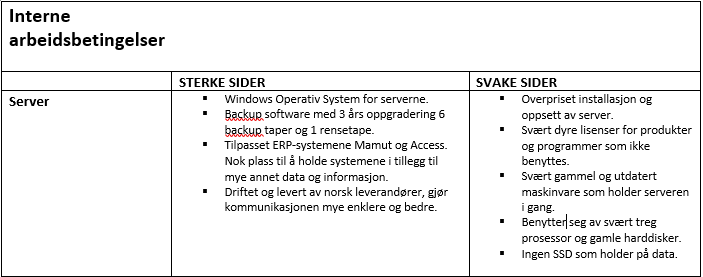
\includegraphics[width=\textwidth]{Bilder/s1.PNG}
%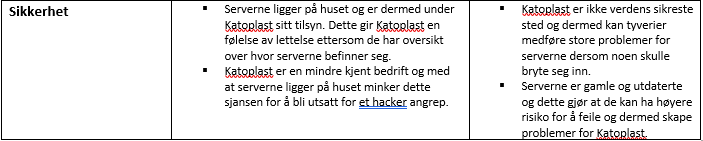
\includegraphics[width=\textwidth]{Bilder/s3.PNG}
%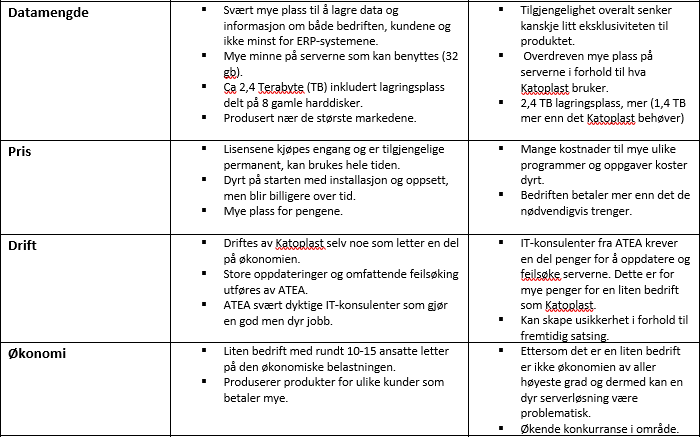
\includegraphics[width=\textwidth]{Bilder/s2.PNG}
%\paragraph{}
%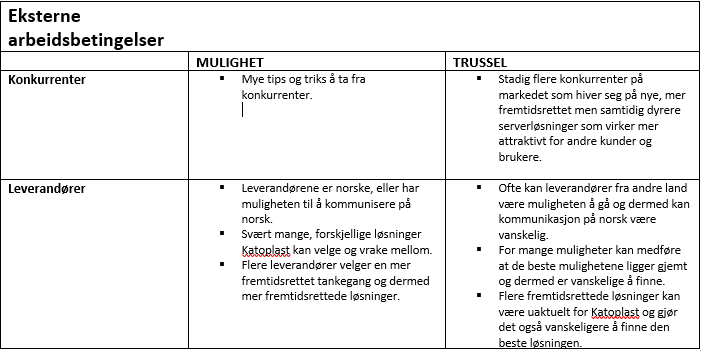
\includegraphics[width=\textwidth]{Bilder/s4.PNG}

% h(ere)t(op) bestemmer hvordan tabellen legger seg (!) betyr den skal forsøke å "force" det.
\begin{longtable}[!ht]{lp{0.4\textwidth}p{0.3\textwidth}} \toprule
	\multicolumn{3}{l}{{\large \textbf{Interne arbeidsbetingelser}}} \\ \midrule
    & \multicolumn{1}{c}{\textbf{Sterke sider}} & \multicolumn{1}{c}{\textbf{Svake sider}} \\ \midrule
    
    \textbf{Server} 
    & % col2 Dette er andre kolonne hvor det står om sterke sider:
    {\scriptsize 
    	\pbox{0.4\textwidth}{%
    	{\tiny \ding{228}} Windows operativsystem for servere. \\ 
    	{\tiny \ding{228}} Backup-software med 3 års oppgradering, 6 backup-taper og 1 rensetape- \\
        {\tiny \ding{228}} Tilpasset ERP-systemene Mamut og Access. \\ 
    	{\tiny \ding{228}} Nok plass til å holde systemene i tillegg til annen data og informasjon. \\
    	{\tiny \ding{228}} Driftet og levert av norske leverandører gjør kommunikasjonen enklere.}} 
    & % col3 Dette er tredje kolonne hvor det står om svake sider:
    {\scriptsize 
    	\pbox{0.3\textwidth}{%
    	{\tiny \ding{228}} Overpriset installasjon og oppsett av server. \\
    	{\tiny \ding{228}} Svært dyre lisenser for programmer som ikke er benyttet. \\
        {\tiny \ding{228}} Svært gammel og utdatert maskinvare som holder serveren i gang. \\
        {\tiny \ding{228}} Benytter seg av svært treg prosessor og gamle harddisker. \\
        {\tiny \ding{228}} Ingen SSD som holder på data.}
    } \\ \cmidrule(l{-0.6in}r){2-3}
    
    \textbf{Sikkerhet} % Nytt tema 
    & % col2 Slik fortsetter det nedover:
    {\scriptsize % setter størrelsen på skriften i denne cellen.
    	\pbox{0.3\textwidth}{% gjør det mulig å bruke linjeskift: \\ inni celler
    	{\tiny \ding{228}} Serverne ligger på huset og er dermed under Katoplasts tilsyn. Dette gir Katoplast følelsen av letterlse ettersom de har oversikt over hvor serverne befinner seg.\\
    	{\tiny \ding{228}} Katoplast er en mindre kjent bedrift og med at serverne ligger på huset minker dette sjangsen for å bli utsatt for et hacker-angrep.
        }
    }
    & % col3 
    {\scriptsize 
    	\pbox{0.3\textwidth}{%
    	{\tiny \ding{228}} Katoplast er ikke verdens sikreste sted og dermed kan tyverier medføre kritiske skader på serverne dersom noen skulle bryte seg inn. \\
    	{\tiny \ding{228}} Serverne er gamle og utdaterte og dette gjør at de kan ha høyere risiko for å feile og dermed skape problemer for Katoplast. 
        }
    } \\ \cmidrule(l{-0.6in}r){2-3}
    
    \textbf{Datamengde}     
    & % col2
    {\scriptsize 
    	\pbox{0.3\textwidth}{%
    	{\tiny \ding{228}} 	Betydelig mer plass til å lagre data og informasjon om både bedriften, kundene og ikke minst for ERP-systemene. \\
    	{\tiny \ding{228}}  Mye minne på serverne som kan benyttes (32 gb).\\
        {\tiny \ding{228}}  	Ca 2,4 Terabyte (TB) inkludert lagringsplass delt på 8 gamle harddisker. \\
        {\tiny \ding{228}} 	Produsert nær de største markedene.  \\
        }
    }
    & % col3 
    {\scriptsize 
    	\pbox{0.3\textwidth}{%
    	{\tiny \ding{228}}	Tilgjengelighet overalt senker eksklusiviteten til produktet.   \\
    	{\tiny \ding{228}} Overdreven mye plass på serverne i forhold til hva Katoplast bruker. \\
        {\tiny \ding{228}} 	2,4 TB lagringsplass, mer (1,4 TB mer enn det Katoplast behøver)  \\
        }
    } \\ \cmidrule(l{-0.6in}r){2-3}
    
    \textbf{Pris}     
    & % col2
    {\scriptsize 
    	\pbox{0.3\textwidth}{%
    	{\tiny \ding{228}}	Lisensene kjøpes engang og er tilgjengelige permanent, kan brukes hele tiden.  \\
    	{\tiny \ding{228}}  	Dyrt på starten med installasjon og oppsett, men blir billigere over tid.\\
        {\tiny \ding{228}} 	Mye plass for pengene. \\
        }
    }
    & % col3 
    {\scriptsize 
    	\pbox{0.3\textwidth}{%
    	{\tiny \ding{228}}  	Mange kostnader til flere ulike programmer og oppgaver koster dyrt. \\
    	{\tiny \ding{228}}	Bedriften betaler mer enn det de nødvendigvis trenger.   \\
        }
    } \\ \cmidrule(l{-0.6in}r){2-3}
    \textbf{Drift}     
    & % col2
    {\scriptsize 
    	\pbox{0.3\textwidth}{%
    	{\tiny \ding{228}} 	Driftes av Katoplast selv noe som letter på økonomien. \\
    	{\tiny \ding{228}} 	Store oppdateringer og omfattende feilsøking utføres av ATEA.  \\
        {\tiny \ding{228}} 	ATEA svært dyktige IT-konsulenter som gjør en god men dyr jobb.  \\
        }
    }
    & % col3 
    {\scriptsize 
    	\pbox{0.3\textwidth}{%
    	{\tiny \ding{228}} 	IT-konsulenter fra ATEA krever store summer for å oppdatere og feilsøke serverne. Dette er for store summer for en liten bedrift som Katoplast.  \\
    	{\tiny \ding{228}} 	Kan skape usikkerhet i forhold til fremtidig satsing.  \\
        }
    } \\ \cmidrule(l{-0.6in}r){2-3}
    \textbf{Økonomi}     
    & % col2
    {\scriptsize 
    	\pbox{0.3\textwidth}{%
    	{\tiny \ding{228}} 	Liten bedrift med rundt 10-15 ansatte letter på den økonomiske belastningen. \\
    	{\tiny \ding{228}} 	Produserer produkter for ulike kunder som betaler mye.  \\ 
        }
    }
    & % col3 
    {\scriptsize 
    	\pbox{0.3\textwidth}{%
    	{\tiny \ding{228}} 	Ettersom det er en liten bedrift er ikke økonomien av aller høyeste grad og dermed kan en dyr serverløsning bli problematisk. \\
    	{\tiny \ding{228}} 	Økende konkurranse i område \\
        }
    } \\ \addlinespace[2mm]\midrule[\heavyrulewidth]\addlinespace[1mm]
    \multicolumn{3}{l}{{\large \textbf{Externe arbeidsbetingelser}}} \\ \midrule
    & \multicolumn{1}{c}{\textbf{Mulighet}} & \multicolumn{1}{c}{\textbf{Trussel}} \\ \midrule
    \textbf{Konkurrenter}     
    & % col2 Til vi kommer hit, hvor nMulighet begynner:
    {\scriptsize 
    	\pbox{0.3\textwidth}{%
    	{\tiny \ding{228}}	Tips og triks å ta fra konkurrenter.   \\
        }
    }
    & % col3 Og her er Trussel:
    {\scriptsize 
    	\pbox{0.3\textwidth}{%
    	{\tiny \ding{228}} 	Stadig flere konkurrenter på markedet som hiver seg på nye, mer fremtidsrettet men samtidig dyrere serverløsninger som virker mer attraktivt for andre kunder og brukere.    \\
        }
    } \\ \cmidrule(l{-0.6in}r){2-3}
    \textbf{Leverandører}     
    & % col2
    {\scriptsize 
    	\pbox{0.3\textwidth}{%
    	{\tiny \ding{228}} 	Leverandørene er norske, eller har muligheten til å kommunisere på norsk. \\
    	{\tiny \ding{228}} 	Svært mange, forskjellige løsninger Katoplast kan velge og vrake mellom.  \\
        {\tiny \ding{228}} 	Flere leverandører velger en mer fremtidsrettet tankegang og dermed mer fremtidsrettede løsninger. \\
        }
    }
    & % col3 
    {\scriptsize 
    	\pbox{0.3\textwidth}{%
    	{\tiny \ding{228}} 	Ofte kan leverandører fra andre land være muligheten å gå og dermed kan kommunikasjon på norsk bli innviklet.   \\
    	{\tiny \ding{228}} 	For mange muligheter kan medføre at de beste mulighetene ligger gjemt og dermed er kompliserte å finne.  \\
        {\tiny \ding{228}}	Flere fremtidsrettede løsninger er uaktuelt for Katoplast og gjør det også vanskeligere å finne den beste løsningen.   \\
        }
    } \\ \cmidrule(l{-0.6in}r){2-3}
\end{longtable}

\section{Spørreundersøkelse}
\paragraph{}For å kartlegge Katoplast sin situasjon i dag, og samtidig også få en oversikt over hvordan Katoplast ønsker at det skal gå for løsningene i fremtiden valgte gruppen å lage en spørreundersøkelse for å kartlegge nettopp dette. Med spørreundersøkelsen ønsket gruppen å finne ut av hvordan daglig lederen rangerer bedriften sin situasjon i dag, og hva slags funksjoner og komponenter ved en server de ønsker skal være med.

\paragraph{} Med hensyn til Katoplast sine kravspesifikasjoner og deres ønsker utarbeidet gruppen en spørreundersøkelse som skulle svare på det gruppen lurte på, og samtidig det gruppen trengte for å kunne gå videre med å finne en passende løsning.

\paragraph{}Undersøkelsen tok for seg en rekke arbeidskrav hvor Katoplast rangerte hvert arbeidskrav på en skala fra 1-10. Gjennom den tilbakemeldingen som ble gitt, valgte gruppen å lage en arbeidskravsanalyse som skulle ta for seg de ulike kravene som bedriften har stilt for prosjektet. Analysen vil gå grundig gjennom de ulikene kravene som er fastsatt for å støtte gruppen i arbeidet med de ulike analysene av løsningene og ikke minst hjelpe gruppen med å finne den riktige løsningen som vil passe for Katoplast. Resultatene på spørreundersøkelsen er som vist på figur 4.1. 

\paragraph{} En arbeidskravsanalyse tar for seg de grunnleggende elementene som er mest fundamental for å løse bedriftens server problem. For å finne best mulig løsningene må arbeidskravene bli sammenlignet opp mot de forskjellige serverløsningene som er mest relevante for en riktig serverløsning.

\paragraph{}I denne analysen er det plukket ut de viktigste elementene for hvordan Katoplast kan finne en serverløsning som passer de best. De blå kolonnene forteller hvor katoplast ligger i dag, og de oransje forteller hva slags krav katoplast ønsker at deres nye server skal legge vekt på.

\begin{figure}[h] % liten h, ikke stor H  ---Ole
\centering
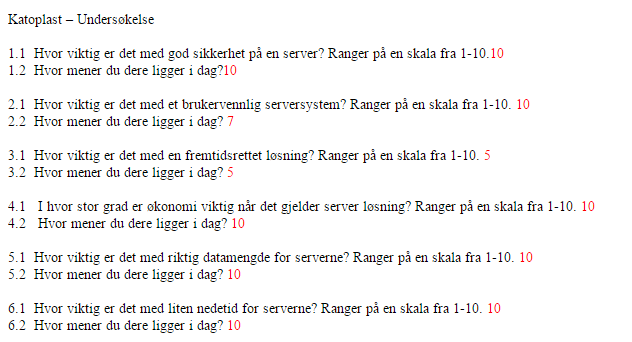
\includegraphics[width=6.5in]{Bilder/sporre.png}
\caption{Spørreundersøkelse}
\end{figure}

\section{Skytjenester}
\subsection{Forbehold} 
\paragraph{} Under blir en rekke sky løsninger presentert som er aktuelle for bedriften Katoplast og som kan eventuelt løse server problemet til Katoplast dersom de skulle ønske å gå for en av disse løsningene. Gruppen er klar over at bedriften ikke ønsker seg en skyløsning, men samtidig forsøker prosjektgruppen å gi Katoplast et nytt syn på skytjenester gjennom de resultatene og den forskningen som har blitt gjort.
\subsection{Technet}
180 000 IT-brukere i 23 land og 6 verdensdeler får skytjenester levert fra Technet sitt datasenter. De 4 største grunnene til å velge komplett skytjenester fra Technet er: 
\begin{enumerate}[noitemsep]
\item Bedriften velger selv applikasjonene de ønsker å bruke, bedriften kan benytte sine fagapplikasjoner i Technet sin skytjeneste. 
\footnote{http://www.xn--skylsninger-jgb.no/skytjenester/}

\item Bedriften kan jobbe hvor som helst. Det vil si alt som behøves er internettforbindelse og en nettleser. Da kan man jobbe fra hele verden.

\item Det kan jobbes på ulike enheter. Det vil si uansett hvilken enhet bedriften bruker, om det er nettbrett, telefon eller datamaskin så vil man ha full tilgang til alle applikasjoner og filer.

\item Hele ansvaret ligger hos Technet. De tar for seg ansvaret for sikkerheten, oppdateringer og at alt fungerer som det skal. 
\end{enumerate}

\paragraph{} Ulike bedrifter har ulike behov. Technet hjelper til med å effektivisere IT-driften i sine skytjenester ut fra bedriftens situasjon i dag og dens fremtidige målsetninger. Technet tilbyr ulike nivåer av skytjenester. Alt fra driftsstøtte og hosting, til sentralisert IT-drift og håndtering av komplette IT-systemer leveres i Technet sin skytjeneste.

\paragraph{} Katoplast kan benytte alle sine fagapplikasjoner i Technet sine skytjenester. Super Office, Visma, Autocad, Mamut, Handyman, Evatic, Solidworks, DI systemer, Maestro, Sticos, PAT, Adobe og Extensor er eksempler på løsninger Technet sine kunder benytter i skytjenesten i dag. \footnote{http://www.technet.no/skytjenester/skytjenester/hvorfor-skytjenester.aspx}

\paragraph{}Lokal IT-drift stiller krav til fysisk nærvær av intern eller ekstern kompetanse. Hvordan håndteres oppgraderinger, virusangrep, backup eller ekstraordinære hendelser etter arbeidstid? Technet kan gjennom skytjenesten tilby profesjonell support døgnet rundt og brukerstøtte direkte på skjermen. I dag er ofte sikkerheten delegert ned til hver datamaskin, som igjen medfører at den største sikkerhetsrisikoen ligger hos den enkelte medarbeider. En skytjeneste gjør det enklere å holde riktig sikkerhetsnivå mot uønsket innlogging, datavirus, sikkert samband, automatisk backup og mot risikoen for å miste data ved brann eller tyveri.

\subsection{Microsoft Azure}
\begin{figure}[H]
\centering

\includegraphics[width=4.2in]{Bilder/azure.png}
\caption{Logoen til Microsoft Azure (Msazurelogo,2015)}
\end{figure}

\paragraph{} Microsoft Azure er en nettsky-basert databehandlings tjeneste lagd av Microsoft. Azure er til for å bygge, utplassere og administrere applikasjoner og tjenester igjennom et globalt nettverk av microsofts egne data-senter. Azure tilbyr blant annet PaaS, IaaS og SaaS tjenester for sine kunder. 
\footnote{https://azure.microsoft.com/nb-no/overview/what-is-iaas/}
\footnote{http://robertgreiner.com/2014/03/windows-azure-iaas-paas-saas-overview/}

\paragraph{} Microsoft sin skyløsning tilbyr en helt egen måte å gjenopprette data på kalt "Site Recovery". Azure tillater brukerne å danne egne gjenopprettingsplaner. Dette er planer som tillater brukerne å planlegge for nødssituasjoner og ikke minst forebygge problemer med data og informasjon. I tillegg tilbyr Azure også automatisk beskyttelse av de virtuelle maskinene som bedriften benytter. Tjenesten er laget for å kunne gjenopprette selv de mest komplekse systemene innenfor en bedrift.
\footnote{https://azure.microsoft.com/nb-no/services/site-recovery/}

\subsection{Amazon Web Services}
\begin{figure}[H]
\centering

\includegraphics[width=4.2in]{Bilder/AWS.png}
\caption{Logoen til Amazon Web Services (Amazon Web Services, 2016)}
\end{figure}
\paragraph{}Amazon Web Services eller AWS er datterselskapet til den kjente Amazon.com. AWS tilbyr en on-demand platform for skytjenester. Fra og med 2016 tilbyr AWS mer enn 70 forskjellige tjenester. Dette inkluderer altså lagring, databaser, analysering, applikasjonstjenester, utplassering, ledelse, utviklerverktøy og networking. Disse tjeneste operer fra 16 forskjellige regioner spredt rundt i verden.
\footnote{ https://aws.amazon.com/application-hosting/benefits/ }
\footnote{ https://npifinancial.com/blog/pros-and-cons-digging-into-amazon-web-services/ }
\footnote{ https://npifinancial.com/blog/pros-and-cons-digging-into-amazon-web-services/ }

\paragraph{}Amazon Elastic Compute Cloud, bedre kjent som Amazon EC2 gir brukerne muligheten til å leie virtuelle datamaskiner hvor brukeren kan kjøre deres egne applikasjoner. EC2 oppmuntrer skalerbar utplassering, dette vil altså si at brukeren kan bruke Amazon sine web-tjenester til å starte et Amazon Machine Image ("AMI") til å konfigurere en virtuell maskin, som inneholder alt ønskelig software. Ved bruk av EC2 betaler du kun for timene du bruker, derav "Elastic". EC2 tilbyr også brukerne tilgang til de 16 forskjellige regionene, dette igjen tillater optimalisering av ventetid ("latency") og et høyt nivå overflødighet.
\footnote{http://docs.aws.amazon.com/AWSEC2/latest/UserGuide/concepts.html}
\footnote{https://aws.amazon.com/ec2/}


\paragraph{}Amazon Simple Storage Service, eller S3 gir brukeren mulighet til å lagre data igjennom web-tjenester. I følge til Amazon er målet med S3 sitt design å skaffe skalering, høy tilgjengelighet og lav ventetid.
\footnote{ https://aws.amazon.com/s3/pricing/ }
\footnote{ https://aws.amazon.com/s3/ }
\footnote{http://docs.aws.amazon.com/AWSEC2/latest/UserGuide/concepts.html}
\paragraph{}Amazon AWS lanserte i 2006, og nå 11 år senere er det i god stand, og høyt rangert som en ren nettsky-basert løsning.


\section{PC Hjelp AS - Intern løsning}
\paragraph{}PC Hjelp AS har gitt gruppen et tilbud. Når man benytter seg av interne servere på huset vil man kunne ha full kontroll over sine egne servere. Man trenger ikke å forholde seg til noen andre, man drifter det meste selv, eller gjennom et IT-team. Serverne blir bygget etter selskapets behov og vil kunne oppgraderes hvis det skulle vært ønsket.
\footnote{http://www.dwuser.com/education/content/why-you-need-a-testing-server-and-how-to-do-it/}



\paragraph{} Når man leter etter en serverløsning som er intern er man avhengig av hardware, software og konsulentarbeid. De forskjellige løsningene prosjektet vil fremstille for Katoplast vil være avhengig av det Katoplast trenger.  Det er essensielt at de løsningene som presenteres ikke har noen svakheter innen hardware eller software opp imot behovet til katoplast. Når det kommer til konsulentjobben kommer den til å bli betalt ut fra timene de trenger for å gjøre jobben gjort, altså ikke for spesifikke egenskaper som er mer relevant for software og hardware. Vesentlig for vurderingen av tilbudet er å vurdere erfaringene til konsulentene i fagfeltet. 
\footnote{http://www.dwuser.com/education/content/why-you-need-a-testing-server-and-how-to-do-it/}
\footnote{http://whatismyipaddress.com/localhost}
\footnote{http://www.episerver.com/learn/resources/blog/udaiappa-ramachandran/the-pros-and-cons-of-cloud-storage/}

\paragraph{} PC Hjelp AS ga prosjektet et tilbud på software, hardware og konsulentarbeidet rundt servere. Disse er tilpasset behovene til Katoplast.
\subsection{Tilbudsinformasjon}
\begin{description}
\item Hardware: Lenovo ThinkServer, 1 x Xeon E3-1225v5, 1x16GB 2x 1TB 3,5* SATA Slim DVD-RW 250W. Pris: 10072,00 kr.
\item Software: Microsoft Windows Server 2012. 
\item Pris: 7192,00 kr
\item Konsulentarbeid: Timespris konsulent Lars Berge. 
\item Pris: 790,00 kr pr. time
\end{description}
  
 
\section{Hybrid Cloud Løsninger}
\subsection{Forbehold}
\paragraph{} Løsningene under tilhører kategorien Hybride Cloud Løsninger. Dette er løsninger som tar for seg den komplekse strukturen og arkitekturen til en hybrid cloud hvor lagringsystemet deles i 2, en public og en private cloud (Figur 4.3). En slik løsning vil Katoplast oppleve en økning i muligheter for lagring og deling av informasjon og ikke minst oppleve en ny form for sikkerhet når det gjelder backup av filer og annen data. I tillegg vil de fleste leverandørene av en Hybrid Cloud være åpne til å gi full støtte til Katoplast med deres installasjon og oppsett av en slik, fremtidsrettet serverløsning. 

\addcontentsline{toc}{section}{Hybrid Cloud Figur}
\section*{}
\begin{figure}[H]
\centering
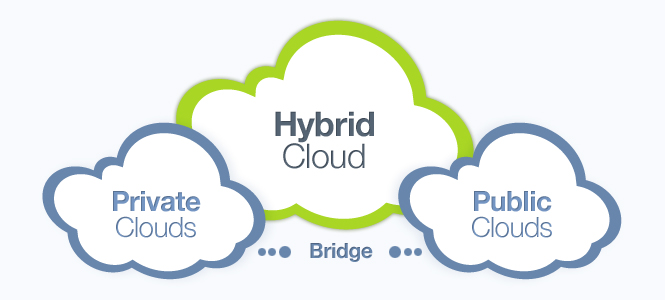
\includegraphics[width=6.5in]{Bilder/Hybrid-cloud.jpg}
\caption{Forenklet figur av en Hybrid Cloud. (Roadmap, 2016)}
\end{figure}

\paragraph{} Hver av disse løsningene har sine fordeler og ulemper som gjør dem både unike og samtidig skiller dem fra hverandre. Deres priser er svært varierende og gruppen har tatt i betraktning de spesifikasjonene og ønskene Katoplast har satt for prosjektet i jakten på å finne den beste løsningen. Flere av løsningene som ble diskutert i gruppen ble utelukket etter en grundig vurdering av pris, tilgjengelighet og sikkerhet. Blant annet ekskluderte gruppen Amazon Web Services (AWS) fra dette prosjektet som følge av de alt for høye kostnadene når det gjelder kjøp og installasjon av en hybrid cloud.

\subsection{Microsoft Azure StorSimple}
\paragraph{} Et av verdens største organisasjon innenfor IT har tatt et stort steg innenfor en fremtidsrettet løsning for bedrifter når det gjelder lagring av informasjon og data. Microsoft sin forskning og dyktige arbeidere har utviklet sin egen løsning for en Hybrid cloud for å skape noe unikt, men samtidig også skape noe som kan benyttes av både store og små bedrifter og ikke minst privatpersoner. Microsoft tilbyr flere, forskjellige former av en Hybrid Cloud og er villige til å tilpasse nettskyen for bedriften akkurat slik de ønsker å ha det. Med deres forskjellige tilbud kan dette bli noe som vil være av interesse for Katoplast. Microsoft Azure StorSimple er den nye formen for hybrid sky som tilbyr bedrifter en helt ny form for lagring av data.
\footnote{https://azure.microsoft.com/nb-no/services/storsimple/}

\addcontentsline{toc}{section}{Microsoft StorSimple}
\section*{}
\begin{figure}[H]
\centering
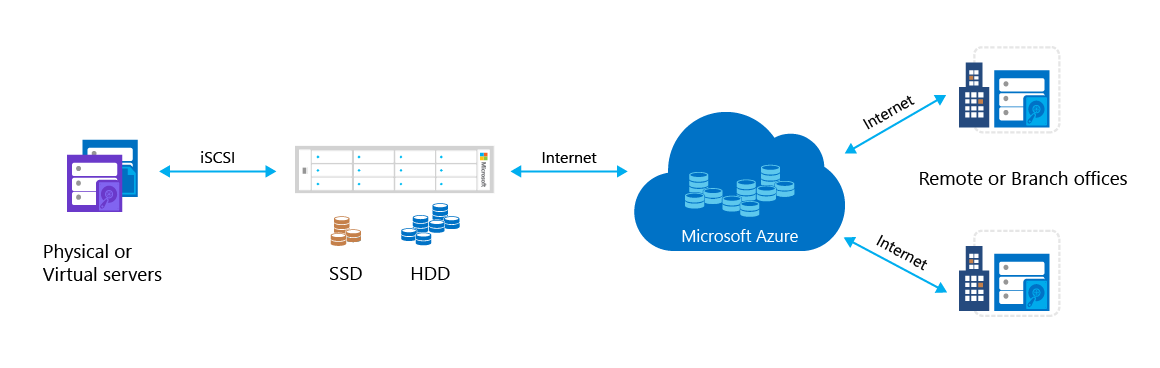
\includegraphics[width=6.5in]{Bilder/storsimple.png}
\caption{StorSimple infrastruktur (StorSimple, 2017)}
\end{figure}

\paragraph{} Med betraktning på Katoplast sine svar på undersøkelsen, har gruppen undersøkt nøye hvilke fordeler som følger med StorSimple. Et av Katoplast sine ønsker var å minke eller automatisere de manuelle, administrative oppgavene som måtte gjennomføres. StorSimple tilbyr nettopp dette med deres automatiserte dataadministrasjon. Med en slik fordel vil Katoplast nå slippe å vedlikeholde store deler av en server, men derimot ha muligheten til å fokusere på andre oppgaver. StorSimple vil arkivere unødvendig data helt automatisk samtidig som den tar seg av vedlikehold av infrastrukturen. Det vil si at de administrative oppgavene som Katoplast arbeider med, blir gjort av StorSimple automatisk. 
\footnote{http://cdn2.hubspot.net/hub/65157/file-1187005090-pdf/StorSimple\_SolutionOverview07-9-14}
\footnote{https://azure.microsoft.com/nb-no/services/storsimple/}

\paragraph{} Et annet konsept med Microsoft sin hybride sky StorSimple er at den legger et stort fokus på backup lagring og nød gjenoppretting av filer og data. Dette er en vesentlig funksjon dersom Katoplast sine servere skulle møte på motgang, nedetid eller at data eventuelt skulle bli slettet eller bli korrupt av ulike årsaker. StorSimple gjør gjenopprettingen av data brukervennlig, og ikke minst tillater den å gjenopprette store datamengder slik at ingenting går tapt. Dermed vil det ikke være noe problem dersom serverne skulle miste informasjon ettersom bedriften vil ha mulighet til å hente tilbake disse. Når det gjelder gjenoppretting av data er dette ofte en smertefull og stressende prosess som må gjøres manuelt på interne servere. StorSimple vil ta seg av alt dette arbeidet og gjøre det så simpelt som mulig for brukerne av nettskyen.
\footnote{https://docs.microsoft.com/en-us/azure/storsimple/storsimple-manage-backup-policies}
\footnote{https://azure.microsoft.com/nb-no/solutions/hybrid-integration/}

\paragraph{} StorSimple er naturligvis et relativt nytt konsept som fortsatt er i utvikling og som vil få mange flere funksjoner i nær fremtid. videre, er det slik at prisene på StorSimple sine tjenester er svært varierende. Tjenesten tilbyr brukere å velge hvor stor lagringsplass de ønsker å kjøpe, om diskene skal være SSD eller HDD og samtidig tilbyr tjenesten ulike abonnement for å tilpasse tjenesten til flere. Basert på den informasjonen som gruppen har samlet fra Katoplast og deres ønsker, har prosjektgruppen funnet en løsning som kan være rimelig, men samtidig kostbar for Katoplast.
\footnote{https://azure.microsoft.com/en-us/pricing/}

\paragraph{} StorSimple deles inn i 2 deler, en fysisk og en virtuell del. Her vil bedrifter og brukere ha muligheten til å velge ulike servere og hvor mange av hver server de ønsker å kjøpe. Hver server har sine, unike fordeler. Modellene på serverne varierer og Microsoft introduserer hele tiden nye modeller. For nå tilbyr Microsoft 2 fysiske apparater, modell 8100 og modell 8600, og 3 virtuelle apparater, modell 8010, modell 8020 og modell 1200. 
\footnote{https://docs.microsoft.com/en-us/azure/storsimple/storsimple-technical-specifications-and-compliance}

\paragraph{} Microsoft tilbyr deres kunder flere måter å kjøpe deres sky tjenester på. Hver av disse metodene er tilpasset ulike kunder og er skapt for å gjøre deres skytjenester tilgjengelig for flere bedrifter og brukere. Et av alternativene siktet mot større bedrifter er en metode kalt "foretaksavtaler". Med en foretaksavtale vil store organisasjoner inngå en avtale med Microsoft om forskuddsbetaling av tjenestene de får.
\footnote{https://azure.microsoft.com/nb-no/pricing/purchase-options/}
\footnote{https://azure.microsoft.com/nb-no/pricing/enterprise-agreement/}

\paragraph{} En annen måte å kjøpe tjenestene på er gjennom Microsoft sitt eget "open-licensing program". Dette er en kjøps metode ment for små til middels-store bedrifter som ønsker å benytte seg av Microsoft sine sky tjenester. Dette er en metode som er simplifisert for bedrifter og som gir større kontroll og oversikt over investeringen. Samtidig tilbyr denne kjøpsmetoden også mindre bedrifter å få deres pris redusert over flere år.
\footnote{https://www.microsoft.com/en-us/licensing/licensing-programs/open-license.aspx}

\paragraph{} En tredje metode for kjøp av nettskyene til Microsoft er gjennom Microsoft partnere. Bedrifter vil ha muligheten til å kjøpe en Microsoft partner som hjelper bedriften med å implementere og opprettholde den beste løsningen for en nettsky. Disse er også kunnskapsrike konsulenter som kan hjelpe med kostnader og andre spørsmål som en bedrift har.
\footnote{https://azure.microsoft.com/nb-no/partners/directory/}

\paragraph{} Microsoft introduserer ofte nye konsepter som de ønsker å virkeliggjøre, og et av deres nye ideer, Nano Server, er fundamentalt for deres cloud og hybride løsninger som de tilbyr brukerne sine.
\footnote{https://www.pluralsight.com/blog/it-ops/microsoft-nano-server-announced}

\subsection{VMware vCloud Air}

\paragraph{} En annen rimelig Hybrid løsning for Katoplast er VMware vCloud Air Hybrid. Dette er VMware sitt svar på en hybrid nettsky hvor datalagring foregår både i skyen og lokalt.VMware gjør det lett for brukere av deres nettsky hvor de samme programvarene benyttes for å gjennomføre lagring og andre type prosesser for både den interne og eksterne nettskyen. I tillegg til dette tillater VMware at prosesser gjennomføres fortløpende uten nedetid, hvor bedriften vil ha mulighet til å legge inn alt av data og informasjon samtidig som de arbeider. Leverandøren tillater også brukere av nettskyen å planlegge tidspunkt hvor de ønsker å legge inn data eller manipulere data. Dette er en nyttig funksjon å ha dersom man ønsker å spare unødvendig arbeid når det gjelder å komme i gang med nettskyen, men at man heller planlegger når man ønsker å gjennomføre endringene. Slik vil nettskyen være forberedt på at det skjer endringer og dermed også unngå problemer.
\footnote{http://www.vmware.com/solutions/cloud-computing.html}
\footnote{http://www.vmware.com/products/cloud-foundation.html}

\addcontentsline{toc}{section}{VMware Hybrid Cloud}
\section*{}
\begin{figure}[H]
\centering
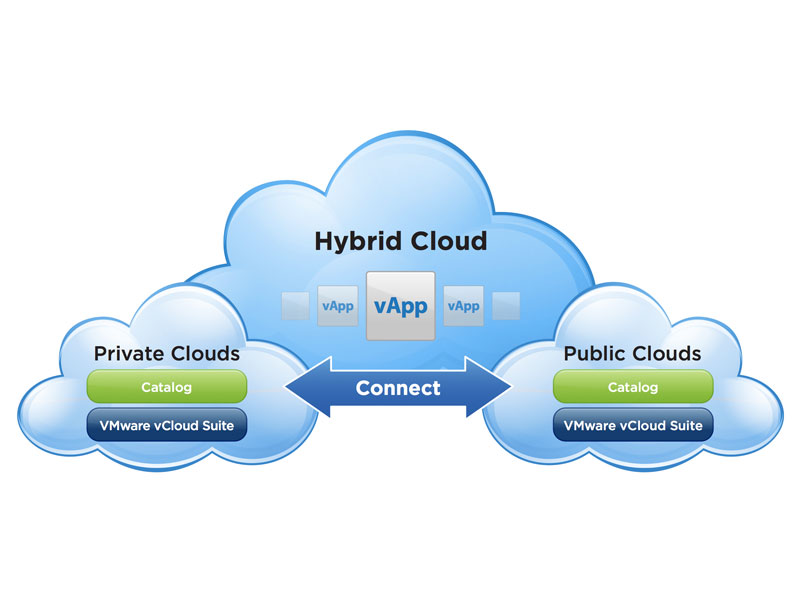
\includegraphics[width=5.5in]{Bilder/vmware.jpg}
\caption{VMware sin Hybride Sky Infrastruktur. Viser hvordan vCloud Suite er koblet opp mot skyene og hvordan disse er koblet sammen. (VMware, 2014)}
\end{figure}


\paragraph{} Videre, så følger VMware et simpelt og brukervennlig tankesett. De ønsker at deres tjenester skal kunne benyttes av så mange som mulig og samtidig være så enkle som mulig. Med tanke på dette har VMware utviklet egne funksjoner, verktøy og innebygde prosesser som deres kunder kan benytte seg av og som tar for seg de administrative oppgavene og andre tunge oppgaver. En fordel med dette er at VMware også støtter flere operativsystemer noe som er avgjørende for Katoplast som kjenner best til Windows Operativ System (OS). 
\footnote{http://www.vmware.com/products/vrealize-suite.html}

\paragraph{} I tillegg har VMware lagt et stort fokus på brukervennlighet når det gjelder deres sky tjenester. Som følge av dette introduserer VMware "vCloud Suite" som er en platform for administrasjon og kontroll av deres sky tjenester. Med vCloud Suite vil mange av de administrative oppgavene gjøres helt automatisk. Tjenesten gjør det også lett for bedrifter å oppgradere eller nedgradere deres hybride løsning bare ved noen få tastetrykk.
\footnote{http://www.vmware.com/products/vrealize-automation.html}
\footnote{http://www.vmware.com/products/vcloud-suite.html}

\paragraph{} Som Microsoft, tilbyr også VMware ulike kjøps metoder når det kommer til deres skyløsninger. I likhet med Microsoft deles også disse i 3 og hver av disse med deres egne fordeler og ulemper, basert på hva bedriften ønsker.
\footnote{https://vcloud.vmware.com/uk/service-offering/pricing-calculator}

\paragraph{} Et av kjøps alternativene som VMware tilbyr kalles "OnDemand" og tilbyr brukere å kun betale for den lagringsplassen de benytter seg av uten å skrive en kontrakt eller noen form for abonnement. For eksempel, dersom Katoplast skulle bruke opp 500gigabyte (gb) lagringsplass ut av 1 terabyte, vil Katoplast kun behøve å betale for de 500 gb de bruker og ikke for de hele 1 TB. Dette alternativet passer best for mindre bedrifter som ikke bruker stort mye plass og dermed kan spare penger på dette.
\footnote{https://vcloud.vmware.com/uk/service-offering/pricing-calculator/on-demand}

\paragraph{} Den andre metoden baserer seg på abonnement. Bedrifter har muligheten til å velge fra ulike abonnement som VMware tilbyr. Fordelen med dette er at man vil ha muligheten til å forutse prisene samt at man vil få tilgang til flere ressurser for å skape en kjappere og bedre server løsning. Et slikt alternativ vil passe for større bedrifter som vet hvor mye lagringsplass de benytter og ønsker tilgangen til flere ressurser for å forbedre deres servere.
\footnote{https://vcloud.vmware.com/uk/service-offering/pricing-calculator/subscription}

\paragraph{} "Horizon Air" er VMware sitt tredje kjøps alternativ og legger vekt på bedrifter som ønsker å benytte seg av virtuelle maskiner og applikasjoner. Velger man Horizon Air vil man inngå et abonnement med VMware hvor man vil ha muligheten til å kjøpe virtuelle maskiner, apper og samtidig ha muligheten til den beste formen av nød gjenoppretting av informasjon og data.
\footnote{http://www.vmware.com/cloud-services/desktop/horizon-cloud-on-premises.html}
\footnote{http://www.vmware.com/cloud-services/desktop/horizon-cloud-hosted.html}

\newpage
\section{Priser}
\paragraph{} Under vil du finne et linjediagram som viser prisene på de ulike bedriftene over flere år. Prisene er sortert på hvert år fra 2017 til utover 2025.
Dette gir bedriften en oversikt over server-budsjettet i fremtiden blant de forskjellige løsningene. 

\addcontentsline{toc}{section}{Microsoft StorSimple}
\section*{}
\begin{figure}[H]
\centering
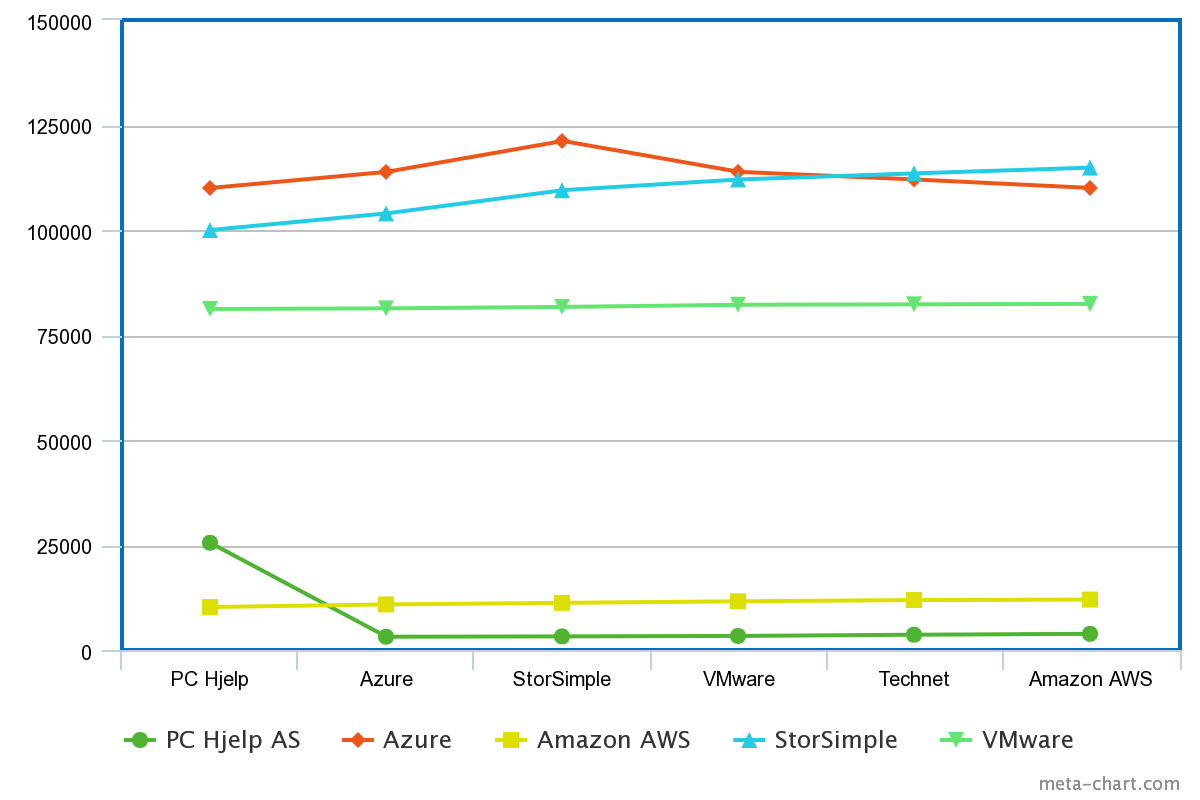
\includegraphics[width=5.5in]{Bilder/priser2.png}
\caption{Serverløsninger Priser}
\end{figure}